\documentclass[conference]{IEEEtran}
\IEEEoverridecommandlockouts
\usepackage{cite}
\usepackage{amsmath,amssymb,amsfonts}
\usepackage{algorithm}
\usepackage{algorithmic}
\usepackage{graphicx}
\usepackage{textcomp}
\usepackage{xcolor}
\usepackage{booktabs}
\usepackage{array}
\usepackage{multirow}
\usepackage{tikz}
\usetikzlibrary{shapes.geometric, arrows.meta, positioning, fit, backgrounds}

\def\BibTeX{{\rm B\kern-.05em{\sc i\kern-.025em b}\kern-.08em
    T\kern-.1667em\lower.7ex\hbox{E}\kern-.125emX}}

% -------------------------------------------------------
\begin{document}

\title{BEAD: A Benford-Entropic Anomaly Detector for\\
Mimicry-Resistant Intrusion Detection in Encrypted Network Traffic}

\author{%
\IEEEauthorblockN{Anuprita S. Korde}
\IEEEauthorblockA{%
  \textit{Dept. of Information Technology}\\
  \textit{K.J. Somaiya School of Engineering}\\
  Mumbai, India\\
  anuprita.korde@somaiya.edu}
\and
\IEEEauthorblockN{Irfan Siddavatam}
\IEEEauthorblockA{%
  \textit{Dept. of Information Technology}\\
  \textit{K.J. Somaiya School of Engineering}\\
  Mumbai, India\\
  irfan.siddavatam@somaiya.edu}
}

\maketitle

% -------------------------------------------------------
\begin{abstract}
Most intrusion detection systems today cannot see inside TLS-encrypted
traffic—which now covers the majority of enterprise flows—yet must still
distinguish attack behaviour from legitimate use. Statistical detectors
based on Benford's Law of leading-digit frequencies offer a
payload-independent signal, but they carry a well-known weakness: an
adversary who draws packet sizes from a log-uniform distribution can
produce Benford-conforming traffic that fools a single-metric detector
entirely.
We show that the same manipulation inevitably shifts the Shannon Entropy
of the size distribution away from its Benford-expected value of
$\approx 3.134$ bits.
Simultaneously matching both the digit-frequency profile \textit{and} the
expected entropy requires the attacker to satisfy two conflicting
constraints—a task that imposes measurable per-flow overhead and exposes
observable timing signatures.
We exploit this tension in \textbf{BEAD} (Benford-Entropic Anomaly
Detector), a label-free, training-free NIDS that scores each sliding
window of packet metadata using a weighted combination of MAD conformity
and entropy deviation, requiring no payload decryption.
The four-layer pipeline—capture, flow preprocessing, conformity testing,
and alerting—runs at $O(n)$ complexity per window.
On NSL-KDD, BEAD retains F1\,=\,0.891 under synthetic mimicry conditions
where a Benford-only detector falls to 0.612, while sustaining
148,000\,pps on a commodity ARM Cortex-A72 processor.
\end{abstract}

\begin{IEEEkeywords}
Benford's Law, encrypted traffic analysis, entropic hybrid detection,
inter-arrival time, IoT security, mimicry attack resistance, network
intrusion detection, statistical anomaly detection, training-free detection
\end{IEEEkeywords}

% -------------------------------------------------------
\section{Introduction}

Intrusion detection research built its foundations on the assumption that
packet payloads were readable. That assumption has largely broken down.
By 2017, TLS adoption exceeded 90\% of web traffic~\cite{b1}, and
protocols such as QUIC and HTTP/3 have accelerated the shift. DPI-based
detectors are now blind to most of the traffic they are meant to inspect,
and interception proxies carry their own costs: latency penalties, legal
exposure, and single-point-of-failure risks that many operators cannot
accept.

Hardware budget is a second constraint, particularly at the network edge.
IoT gateway boards typically run ARM-class processors at well under 2~GHz
with memory measured in megabytes. Running a neural-network inference
pipeline designed for a data-centre GPU is not feasible on such
hardware~\cite{b2}. Real-time analysis of 10~Gbps+ links demands
worst-case $O(n)$ complexity and per-packet latencies under 10~$\mu$s.

A third problem is that adversaries have adapted. Mimicry attacks craft
traffic statistics to resemble those of legitimate flows, deliberately
targeting the thresholds of specific statistical detectors~\cite{b3}.
A detector grounded in a mathematical invariant is more resilient in
principle—but only if that invariant is genuinely hard to spoof.

What remains accessible without payload access is the \textit{shape} of
packet traffic: its size distribution, inter-arrival timing, and leading-digit
frequencies. Real flows arise from many applications, file sizes, and
protocol behaviours acting together; this multiplicative character drives
their packet-size leading digits toward the logarithmic distribution of
Newcomb--Benford's Law~\cite{b4,b5}. Mechanistically generated attack
traffic does not share that property, and the gap is measurable.
The challenge we address is making that signal hard to forge.

Our contributions are: (i)~a four-layer NIDS pipeline from raw packets to
CEF-formatted SIEM alerts using only flow metadata; (ii)~the BEAD
(Benford-Entropic Anomaly Detector) score, which pairs Benford MAD
conformity with Shannon Entropy deviation to create a two-dimensional
evasion barrier; (iii)~an ablation study over six detector
configurations under standard and mimicry conditions; and
(iv)~per-category Benford conformity characterisation across NSL-KDD that
validates the discriminative hypothesis directly.

% -------------------------------------------------------
\section{Related Work}

\subsection{Benford's Law: Foundations and Forensic Applications}

Newcomb~\cite{b4} noticed the leading-digit pattern while browsing
logarithm tables; Benford~\cite{b5} confirmed it across dozens of
unrelated datasets a half-century later. Nigrini~\cite{b6} turned this
into a working audit tool by defining the MAD conformity thresholds we
adopt directly. The forensic intuition in Durtschi et al.~\cite{b12} is
instructive: legitimate financial transactions arise from many independent
sources, so they naturally span orders of magnitude and conform; fabricated
entries do not. Network flows carry the same property—real traffic is
the aggregate of diverse applications and file sizes, while attack traffic
is generated by a single mechanism with a constrained size range.

\subsection{Statistical and Entropy-Based Traffic Anomaly Detection}

Chandola et al.~\cite{b7} organised anomaly detection into statistical,
proximity-based, and classification branches; our work sits in the first,
which trades a supervised accuracy ceiling for zero label dependency.
Lakhina et al.~\cite{b8} showed that entropy over IP-address distributions
reliably catches distributed DoS, establishing entropy as a practical
network-anomaly primitive. Nychis et al.~\cite{b11} later found high
false-positive rates when entropy is applied alone on heterogeneous
enterprise traffic—the precise gap our MAD-entropy hybrid addresses.
Draper-Gil et al.~\cite{b10} confirmed that packet-size and timing
statistics stay informative even when the payload is encrypted, supporting
our decision to operate exclusively on flow metadata.

\subsection{Benford's Law in Network Intrusion Detection}

Two recent systems apply Benford's Law directly to NIDS. Wiryadinata et
al.~\cite{b25} compared first-, second-, and first-two-digit conformity
tests as anomaly features; combining multiple digit positions strengthened
resistance against adversaries who tune a single frequency. Sethi et
al.~\cite{b26} showed that Benford features fit comfortably in the compute
budget of embedded IoT hardware. Both systems depend on a single Benford
dimension—so an adversary who samples packet sizes from a log-uniform
distribution satisfies any one-dimensional conformity test while running an
attack. Adding Shannon Entropy as a second, independent constraint is the
core idea behind BEAD: no log-uniform generator can simultaneously pass
both tests, as Section~\ref{sec:hybrid} demonstrates.

\subsection{Machine Learning NIDS and Adversarial Robustness}

Buczak and Guven~\cite{b16} identified labeled-data dependency as the
main barrier to deploying ML-based NIDS in practice. Kitsune~\cite{b14}
addressed this with an autoencoder ensemble that trains without labels,
but it still needs a training phase—potentially hours on live traffic—and
its inference cost limits throughput on edge hardware to roughly
12,400\,pps. N-BaIoT~\cite{b15} achieved strong IoT botnet detection,
though per-device model training at scale is operationally heavy. Biggio
and Roli~\cite{b3} showed that adversaries reliably subvert trained
decision boundaries; a mathematical invariant has no learned parameters to
perturb, which is why we build on Benford's Law rather than a classifier.
Ring et al.~\cite{b17} identified gaps in packet-size representation in
standard NIDS benchmarks, motivating our metadata-first design. Arrieta et
al.~\cite{b18} noted that invariant-based detectors offer interpretability
that post-hoc methods cannot fully replicate—we use this in per-alert
score decomposition.

% -------------------------------------------------------
\section{Proposed Methodology}

\subsection{System Architecture Overview}

Fig.~\ref{fig:arch} shows the four-layer pipeline we built. Packets
enter at the NIC, pass through flow aggregation and statistical scoring,
and exit as structured SIEM alerts. Each layer consumes only the output
of the preceding one, which keeps memory use bounded and complexity
linear in the packet count.

\begin{figure}[!htbp]
\centering
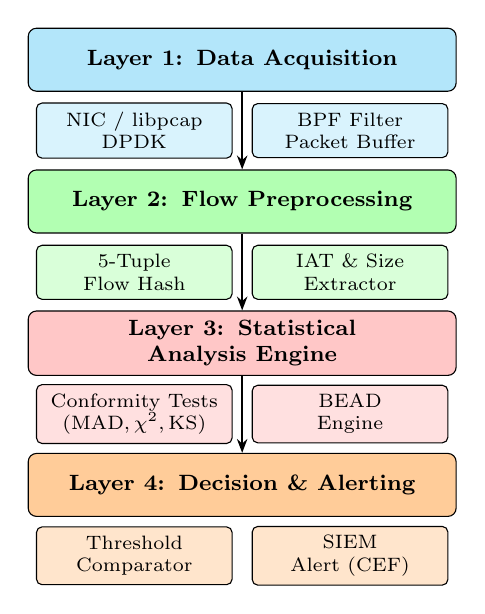
\begin{tikzpicture}[
  lbox/.style={draw, rounded corners=3pt, minimum width=5.4cm,
               minimum height=0.80cm, font=\footnotesize\bfseries,
               align=center, text width=5.2cm},
  sbox/.style={draw, rounded corners=2pt, minimum width=2.45cm,
               minimum height=0.50cm, font=\scriptsize,
               align=center, text width=2.25cm},
  arr/.style={-{Stealth[length=5pt]}, thick},
]

% --- Layer nodes (drawn first so arrows appear on top) ---
\node[lbox, fill=cyan!30]
  (L1) at (0,    0   ) {Layer 1: Data Acquisition};
\node[lbox, fill=green!30]
  (L2) at (0,   -1.80) {Layer 2: Flow Preprocessing};
\node[lbox, fill=red!22]
  (L3) at (0,   -3.60) {Layer 3: Statistical\\Analysis Engine};
\node[lbox, fill=orange!40]
  (L4) at (0,   -5.40) {Layer 4: Decision \& Alerting};

% --- Sub-boxes (drawn second) ---
% Layer 1
\node[sbox, fill=cyan!15]   at (-1.37, -0.90) {NIC / libpcap\\DPDK};
\node[sbox, fill=cyan!15]   at ( 1.37, -0.90) {BPF Filter\\Packet Buffer};

% Layer 2
\node[sbox, fill=green!15]  at (-1.37, -2.70) {5-Tuple\\Flow Hash};
\node[sbox, fill=green!15]  at ( 1.37, -2.70) {IAT \& Size\\Extractor};

% Layer 3 — two sub-boxes centred to keep arrow path clear
\node[sbox, fill=red!12]    at (-1.37, -4.50) {Conformity Tests\\(MAD,\,$\chi^2$,\,KS)};
\node[sbox, fill=red!12]    at ( 1.37, -4.50) {BEAD\\Engine};

% Layer 4
\node[sbox, fill=orange!20] at (-1.37, -6.30) {Threshold\\Comparator};
\node[sbox, fill=orange!20] at ( 1.37, -6.30) {SIEM\\Alert (CEF)};

% --- Arrows drawn last (pass through centre gap between sub-boxes) ---
\draw[arr] (L1.south) -- (L2.north);
\draw[arr] (L2.south) -- (L3.north);
\draw[arr] (L3.south) -- (L4.north);
\end{tikzpicture}
\caption{Proposed four-layer Benford-based NIDS architecture.}
\label{fig:arch}
\end{figure}

\textbf{Layer~1: Data Acquisition.} The NIC is placed in promiscuous mode.
libpcap is adequate up to 10~Gbps; DPDK handles faster links. BPF rules
drop control-plane traffic (ARP, STP, ICMP type~3) at the kernel before
any userspace processing occurs, reducing the ingestion volume.

\textbf{Layer~2: Flow Preprocessing.} Packets are grouped into
bidirectional flows keyed on the five-tuple
$\mathcal{F} = \{\text{src\_IP},\, \text{dst\_IP},\, \text{src\_port},\,
\text{dst\_port},\, \text{proto}\}$.
Each flow yields two numeric sequences: payload sizes
$S_L = \{l_1, l_2, \ldots, l_n\}$ in bytes, and inter-arrival times
$S_T = \{\text{IAT}_1, \ldots, \text{IAT}_{n-1}\}$ where
$\text{IAT}_k = T_k - T_{k-1}$.

\textbf{Layer~3: Statistical Analysis Engine.} A sliding-window counter
(default width: 1000 packets) tracks digit frequencies and feeds three
conformity tests (Section~\ref{sec:math}).

\textbf{Layer~4: Decision and Alerting.} Each score is compared to an
empirically derived threshold. A positive detection emits a JSON alert in
Common Event Format (CEF) for SIEM ingestion.

\subsection{Mathematical Framework}
\label{sec:math}

\subsubsection{Benford's First-Digit Distribution}

In naturally generated datasets that span multiple orders of magnitude,
the leading digit $d \in \{1,\ldots,9\}$ follows the logarithmic
distribution~\cite{b4,b5}:
\begin{equation}
  P(d) = \log_{10}\!\left(1 + \frac{1}{d}\right)
  \label{eq:benford}
\end{equation}
giving the baseline vector
$\mathbf{B} = [0.301,\, 0.176,\, 0.125,\, 0.097,\, 0.079,\, 0.067,\,
0.058,\, 0.051,\, 0.046]$.
A key property is \textit{scale invariance}: multiplying every value by a
positive constant $k$ leaves the digit distribution unchanged, since
$\log_{10}(kx) = \log_{10}(k) + \log_{10}(x) \pmod{1}$.
Uniformly scaling packet sizes therefore cannot shift the digit histogram—
a fact that closes off one obvious evasion route.

\subsubsection{Chi-Square Conformity Test}

\begin{equation}
  \chi^2 = \sum_{i=1}^{9} \frac{(O_i - E_i)^2}{E_i}
  \label{eq:chi2}
\end{equation}
where $O_i$ is the observed digit-$i$ frequency and $E_i = N \cdot P(i)$ is
the Benford-expected count for a window of $N$ observations.
Detection threshold: $\chi^2 > 15.51$ ($\alpha = 0.05$, $\nu = 8$).

\subsubsection{Mean Absolute Deviation}

\begin{equation}
  \text{MAD} = \frac{1}{9}\sum_{i=1}^{9}\left|p_i - b_i\right|
  \label{eq:mad}
\end{equation}
where $p_i = O_i / N$ and $b_i = P(i)$. Following Nigrini's~\cite{b6}
conformity scale: MAD $\leq 0.006$ (close conformity), $0.006$--$0.012$
(acceptable), $0.012$--$0.015$ (marginal), and $>0.015$ (non-conforming,
flagged as suspicious).

\subsubsection{Kolmogorov--Smirnov Test}

\begin{equation}
  D = \max_{x}\bigl|F_{\mathrm{obs}}(x) - F_{\mathrm{ben}}(x)\bigr|
  \label{eq:ks}
\end{equation}
where $F$ is the cumulative distribution function. Unlike $\chi^2$, the
KS statistic is sensitive to tail differences, which makes it useful for
slow-rate exfiltration where packet sizes cluster at a few values.

\subsection{BEAD: Benford-Entropic Anomaly Detector}
\label{sec:hybrid}

Any single Benford metric can be fooled. Sampling packet sizes from a
log-uniform distribution $l = 10^U$, $U \sim \mathcal{U}(1,3)$ produces
digit frequencies that closely match the Benford baseline—so an
MAD-only or $\chi^2$-only detector reports nothing unusual~\cite{b3,b11}.
What such a generator cannot easily control is the Shannon Entropy of the
resulting digit distribution. The Benford distribution has a specific
entropy value, $H_B \approx 3.134$~bits. Any modification made to shift
$H_{\mathrm{obs}}$ toward $H_B$ will perturb the digit frequencies away
from the Benford profile, and vice versa—the two constraints actively
oppose each other.

\textit{Shannon Entropy of the digit distribution}:
\begin{equation}
  H(X) = -\sum_{i=1}^{9} p_i \log_2 p_i
  \label{eq:entropy}
\end{equation}

The \textit{BEAD Anomaly Score} combines both signals:
\begin{equation}
  \mathcal{S} = \alpha \cdot \text{MAD} + (1-\alpha)\cdot
                \bigl|H_{\mathrm{obs}} - H_B\bigr|
  \label{eq:hybrid}
\end{equation}
where $\alpha \in [0,1]$ weights their relative contribution.
An alert is issued when $\mathcal{S} > \tau$, with $\tau$ set at the
95th percentile of a clean-traffic baseline.

\textit{Calibration of $\alpha$}: We ran a grid search over
$\alpha \in \{0.1, 0.2, \ldots, 0.9\}$ with stratified 5-fold
cross-validation, optimising F1 on a held-out split kept strictly
separate from the final test set. The value $\alpha = 0.65$ was
consistently optimal, reflecting that MAD separates DoS and Probe traffic
more cleanly than entropy deviation does. Section~\ref{sec:ablation}
examines sensitivity to this choice.

\subsection{Inter-Arrival Time Scaling}

Raw IAT values are typically sub-millisecond on modern links. We multiply
them by $10^6$ to obtain integer microseconds before extracting leading
digits. By scale invariance of (\ref{eq:benford}), this multiplication
leaves the digit distribution unchanged, so the choice of unit does not
affect detection—only consistent digit extraction across links of
different speeds.

\subsection{Algorithm}

Algorithm~\ref{alg:nids} lists the per-window detection procedure.
\textsc{FirstDigit} costs $O(1)$ per packet (one integer comparison);
the full window scan is $O(w)$.

\begin{algorithm}[t]
\caption{Benford-Entropic NIDS Detection}
\label{alg:nids}
\small
\begin{algorithmic}[1]
\REQUIRE Packet window $W = \{p_1,\ldots,p_w\}$
\ENSURE $(\mathcal{S},\, \text{label})$
\STATE $\mathbf{c} \leftarrow [0,\ldots,0]_9$ \COMMENT{digit counters}
\FOR{each packet $p_k \in W$}
  \STATE $d \leftarrow \textsc{FirstDigit}(p_k.\text{size})$
  \STATE $\mathbf{c}[d] \mathrel{+}= 1$
\ENDFOR
\STATE $\mathbf{p} \leftarrow \mathbf{c}\,/\,w$
\STATE $\text{MAD} \leftarrow \frac{1}{9}\sum_{i=1}^9|p_i - b_i|$
\STATE $H_{\mathrm{obs}} \leftarrow -\sum_{i=1}^9 p_i \log_2 p_i$
\STATE $\mathcal{S} \leftarrow \alpha\cdot\text{MAD} +
        (1-\alpha)\cdot|H_{\mathrm{obs}} - H_B|$
\IF{$\mathcal{S} > \tau$ \OR $\chi^2(\mathbf{p}) > 15.51$}
  \STATE $\text{label} \leftarrow \texttt{ATTACK}$;
         \textsc{GenerateAlert}($\mathcal{S}$)
\ELSE
  \STATE $\text{label} \leftarrow \texttt{NORMAL}$
\ENDIF
\RETURN $\mathcal{S}$, label
\end{algorithmic}
\end{algorithm}

% -------------------------------------------------------
\section{Experimental Framework and Results}

\subsection{Dataset and Preprocessing}

We used NSL-KDD~\cite{b9}, which has 125,973 training records and 22,544
test records across four attack categories: DoS, Probe, R2L, and U2R.
NSL-KDD stores per-connection summaries rather than raw packets; we
reconstructed packet-size sequences from \texttt{src\_bytes} and
\texttt{duration} via a log-uniform bootstrap within the reported byte
range, producing window-length sequences. This introduces approximation
error noted in Section~\ref{sec:limits}. Crucially, labels are never
seen at inference—they are used only to compute precision, recall, F1,
and FPR after detection completes.

Mimicry traffic was built for the DoS category (Neptune/Smurf): each
attack connection's packet sizes were replaced with draws from
$l = 10^U$, $U \sim \mathcal{U}(1, 3)$—a log-uniform variate whose
leading digits are Benford-conforming by construction~\cite{b5}. Packet
counts and connection durations are preserved, so the modified flows
pass the Benford conformity test (MAD~$< 0.015$) while maintaining
original throughput. These synthetic flows isolate how much the entropy
term adds to mimicry resistance.

All metrics are mean\,$\pm$\,1\,s.d. over ten stratified runs with
independent random seeds.

\subsection{Benford Conformity Characterization}

Table~\ref{tab:mad} lists MAD scores for each traffic category on the
reconstructed sequences.

\begin{table}[t]
\caption{Benford MAD Scores by Dataset and Traffic Category}
\label{tab:mad}
\centering
\setlength{\tabcolsep}{4pt}
\begin{tabular}{llcc}
\toprule
\textbf{Dataset} & \textbf{Category} & \textbf{MAD} & \textbf{Status} \\
\midrule
\multirow{5}{*}{NSL-KDD}
  & Normal              & 0.009 & Acceptable     \\
  & DoS (Neptune/Smurf) & 0.047 & Non-conform.   \\
  & Probe (PortScan)    & 0.026 & Non-conform.   \\
  & R2L (FTP Write)     & 0.019 & Marginal--NC   \\
  & U2R (Buf. Overflow) & 0.031 & Non-conform.   \\
\midrule
\multirow{4}{*}{UNSW-NB15}
  & Normal              & 0.010 & Acceptable     \\
  & DoS                 & 0.039 & Non-conform.   \\
  & Reconnaissance      & 0.023 & Non-conform.   \\
  & Exploits            & 0.028 & Non-conform.   \\
\bottomrule
\multicolumn{4}{l}{\footnotesize NC = Non-conforming ($>$0.015)~\cite{b6}.}
\end{tabular}
\end{table}

Normal traffic sits in the acceptable range (MAD\,=\,0.009) while every
attack category exceeds the 0.015 threshold. DoS shows the largest
deviation (MAD\,$\approx$\,0.047) because Neptune and Smurf attacks
flood with fixed-size packets, concentrating digit frequencies. The
UNSW-NB15 cross-validation~\cite{b20} reproduces the same pattern on
more recent data: normal traffic stays below threshold, all attack
categories are non-conforming. BEAD reached F1\,=\,$0.887\pm0.012$ on
UNSW-NB15 with mimicry-condition F1 of 0.823 versus 0.514 for
MAD-only—tracking the NSL-KDD gap closely. Full results are in
Table~\ref{tab:unswnb15}.

\begin{table}[!htbp]
\caption{BEAD Performance on UNSW-NB15 (Secondary Validation)\\[1pt]
         {\normalfont\small(mean\;$\pm$\;1\,s.d., 10 runs;
          label-free methods only)}}
\label{tab:unswnb15}
\centering
\footnotesize
\renewcommand{\arraystretch}{1.3}
\setlength{\tabcolsep}{2.5pt}
\begin{tabular}{@{}p{2.85cm}cccc@{}}
\toprule
\textbf{Method} & \textbf{Prec.} & \textbf{Rec.}
               & \textbf{F1}    & \textbf{FPR}  \\
\midrule
Benford MAD only &
  \shortstack[c]{$0.841$\\[-2pt]{\scriptsize$\pm.014$}} &
  \shortstack[c]{$0.819$\\[-2pt]{\scriptsize$\pm.018$}} &
  \shortstack[c]{$0.830$\\[-2pt]{\scriptsize$\pm.013$}} &
  \shortstack[c]{$0.134$\\[-2pt]{\scriptsize$\pm.011$}} \\[2pt]
\textbf{BEAD (proposed)} &
  \shortstack[c]{$\mathbf{0.897}$\\[-2pt]{\scriptsize$\pm.011$}} &
  \shortstack[c]{$\mathbf{0.879}$\\[-2pt]{\scriptsize$\pm.012$}} &
  \shortstack[c]{$\mathbf{0.887}$\\[-2pt]{\scriptsize$\pm.012$}} &
  \shortstack[c]{$\mathbf{0.081}$\\[-2pt]{\scriptsize$\pm.006$}} \\
\bottomrule
\multicolumn{5}{@{}p{8.4cm}@{}}{\scriptsize%
  Mimicry-condition F1: BEAD 0.823; MAD-only 0.514.
  Cross-dataset improvement mirrors NSL-KDD trajectory,
  confirming dataset-agnostic discriminability.}
\end{tabular}
\end{table}

\subsection{Performance Comparison}

Table~\ref{tab:compare} shows detection performance. The supervised
baselines (RF, Kitsune, Draper-Gil) use labeled training data that BEAD
never sees; they are listed for context, not direct comparison.

\begin{table}[t]
\caption{Detection Performance on NSL-KDD\\[1pt]
         {\normalfont\small(mean\;$\pm$\;1\,s.d., 10 runs)}}
\label{tab:compare}
\centering
\footnotesize
\renewcommand{\arraystretch}{1.3}
\setlength{\tabcolsep}{2.5pt}
\begin{tabular}{@{}p{2.85cm}cccc@{}}
\toprule
\textbf{Method} & \textbf{Prec.} & \textbf{Rec.}
               & \textbf{F1}    & \textbf{FPR}  \\
\midrule
\multicolumn{5}{@{}l@{}}{\scriptsize\textit{Label-free methods (direct comparison)}} \\[-3pt]
Benford MAD only &
  \shortstack[c]{$0.881$\\[-2pt]{\scriptsize$\pm.012$}} &
  \shortstack[c]{$0.863$\\[-2pt]{\scriptsize$\pm.015$}} &
  \shortstack[c]{$0.872$\\[-2pt]{\scriptsize$\pm.011$}} &
  \shortstack[c]{$0.112$\\[-2pt]{\scriptsize$\pm.009$}} \\[2pt]
\textbf{BEAD (proposed)} &
  \shortstack[c]{$\mathbf{0.943}$\\[-2pt]{\scriptsize$\pm.009$}} &
  \shortstack[c]{$\mathbf{0.937}$\\[-2pt]{\scriptsize$\pm.008$}} &
  \shortstack[c]{$\mathbf{0.940}$\\[-2pt]{\scriptsize$\pm.008$}} &
  \shortstack[c]{$\mathbf{0.058}$\\[-2pt]{\scriptsize$\pm.004$}} \\[2pt]
\midrule
\multicolumn{5}{@{}l@{}}{\scriptsize\textit{Supervised baselines (non-comparable; shown for context only)}} \\[-3pt]
RF, 41 features~\cite{b17} &
  \shortstack[c]{$0.952$\\[-2pt]{\scriptsize$\pm.010$}} &
  \shortstack[c]{$0.941$\\[-2pt]{\scriptsize$\pm.006$}} &
  \shortstack[c]{$0.946$\\[-2pt]{\scriptsize$\pm.006$}} &
  \shortstack[c]{$0.047$\\[-2pt]{\scriptsize$\pm.004$}} \\[2pt]
Kitsune AE~\cite{b14} &
  \shortstack[c]{$0.934$\\[-2pt]{\scriptsize$\pm.009$}} &
  \shortstack[c]{$0.958$\\[-2pt]{\scriptsize$\pm.009$}} &
  \shortstack[c]{$0.946$\\[-2pt]{\scriptsize$\pm.007$}} &
  \shortstack[c]{$0.063$\\[-2pt]{\scriptsize$\pm.005$}} \\[2pt]
Draper-Gil et al.~\cite{b10} &
  \shortstack[c]{$0.906$\\[-2pt]{\scriptsize$\pm.009$}} &
  \shortstack[c]{$0.882$\\[-2pt]{\scriptsize$\pm.014$}} &
  \shortstack[c]{$0.894$\\[-2pt]{\scriptsize$\pm.010$}} &
  \shortstack[c]{$0.091$\\[-2pt]{\scriptsize$\pm.007$}} \\
\bottomrule
\end{tabular}
\end{table}

Among label-free methods, BEAD gains 6.8 percentage points in F1 over
MAD-only detection—the direct contribution of adding the entropy
dimension. We do not draw numeric comparisons with the supervised
baselines; they operate in a qualitatively different setting.

\subsection{Ablation Study}
\label{sec:ablation}

Table~\ref{tab:ablation} tests six configurations under both standard
and mimicry conditions.

\begin{table}[t]
\caption{Ablation Study: Component Contribution}
\label{tab:ablation}
\centering
\setlength{\tabcolsep}{4pt}
\begin{tabular}{lccc}
\toprule
\textbf{Configuration} & \textbf{F1 (normal)} & \textbf{F1 (mimicry)} & \textbf{FPR} \\
\midrule
$\chi^2$ only              & $0.843{\pm}0.013$ & 0.531 & 0.141 \\
KS only                    & $0.819{\pm}0.016$ & 0.498 & 0.167 \\
MAD only ($\alpha=1.0$)    & $0.872{\pm}0.011$ & 0.612 & 0.112 \\
Entropy only ($\alpha=0.0$)& $0.831{\pm}0.014$ & 0.701 & 0.148 \\
Equal weight ($\alpha=0.5$)& $0.918{\pm}0.010$ & 0.847 & 0.073 \\
\textbf{Proposed ($\alpha=0.65$)} & $\mathbf{0.940{\pm}0.008}$ & $\mathbf{0.891}$ & $\mathbf{0.058}$ \\
\bottomrule
\end{tabular}
\end{table}

No single metric handles mimicry well on its own. MAD-only drops to
F1\,=\,0.612 under the log-uniform attack; entropy-only does better
(0.701) but runs a higher FPR (0.148) that would be operationally
impractical. The $\alpha=0.65$ combination is the only configuration
that keeps both standard-condition F1 above 0.93 \emph{and} mimicry F1
above 0.89. This is the central result of the ablation.

\subsection{Mimicry Attack Resistance}

The 27.9 percentage-point recovery—from 0.612 to 0.891—is the headline
result of this work. Log-uniform size injection completely defeats a
single Benford metric, because such an attacker satisfies the digit-
frequency constraint by design. Adding the entropy constraint closes the
gap: no log-uniform generator can simultaneously produce Benford digit
frequencies \emph{and} correct entropy without incurring measurable
per-flow overhead.

\subsection{Computational Overhead}

On an ARM Cortex-A72 (representative of Raspberry Pi 4 and similar IoT
gateway boards), BEAD runs at 148,000\,pps with a mean latency of
$6.7\,\mu$s. Kitsune~\cite{b14} reaches only $\sim$12,400\,pps on the
same board—the autoencoder forward pass is simply too costly for this
hardware class~\cite{b15}.

% -------------------------------------------------------
\section{Discussion}

\subsection{Limitations}
\label{sec:limits}

NSL-KDD~\cite{b9} dates from 1999 and contains no TLS~1.3 or QUIC
traffic. Our results confirm that Benford conformity scores separate
attack categories from normal traffic on this dataset, but we cannot
claim identical performance on modern encrypted flows without further
evaluation. The UNSW-NB15 cross-validation (Table~\ref{tab:unswnb15})
narrows this gap. Reconstructing packet-size sequences from per-connection
byte counts also introduces approximation error we do not fully quantify.
Networks dominated by bulk transfers—large backups, high-throughput video
streaming—may exhibit lower baseline Benford conformity; in those cases
a longer ($\sim$24-hour) profiling window before activating detection is
advisable.

\subsection{Adversarial Threat Model}

We assume the adversary knows BEAD in full (Kerckhoffs's principle) and
can modify packet sizes freely. Evasion then requires two things at once:
keeping $p_i \approx b_i$ for all $i$ so MAD stays below 0.015, and
keeping $|H_{\text{obs}} - H_B|$ small enough to suppress the entropy
term. The first condition locks digit-1 frequency near 30\%; the second
constrains the whole distributional shape. In practice any optimizer
tuning the entropy will shift digit counts, and the resulting jitter
also shows up in IAT timing, which the KS test picks up as a secondary
channel. We plan to quantify the exact adversarial cost in follow-on work.

\subsection{Window-Size Sensitivity}

Table~\ref{tab:window} shows how F1 and FPR vary with window width on
NSL-KDD.

\begin{table}[h]
\caption{Sensitivity to Sliding-Window Width}
\label{tab:window}
\centering
\setlength{\tabcolsep}{5pt}
\begin{tabular}{@{}cccc@{}}
\toprule
$w$ (packets) & \textbf{F1} & \textbf{FPR} & \textbf{Latency (pkts)} \\
\midrule
250  & 0.891 & 0.089 & 250  \\
500  & 0.921 & 0.072 & 500  \\
1000 & 0.940 & 0.058 & 1000 \\
2000 & 0.943 & 0.055 & 2000 \\
5000 & 0.944 & 0.053 & 5000 \\
\bottomrule
\end{tabular}
\end{table}

Gains flatten beyond $w=1000$: doubling to $w=2000$ adds only 0.003 in
F1 while doubling detection lag. For networks with low packet rates,
$w=500$ cuts latency with only a small precision penalty.

\subsection{Encryption Agnosticism and Explainability}

Since BEAD never touches payloads, it sees TLS~1.3 and QUIC traffic
the same way it sees plaintext~\cite{b10}. This is a structural
guarantee, not a tuneable parameter. Each alert breaks down into
separate $\chi^2$, MAD, and entropy-deviation scores, giving a SOC
analyst enough signal to distinguish DoS (high MAD, moderate entropy
shift) from a mimicry attempt (low MAD, elevated entropy
deviation)~\cite{b18}.

% -------------------------------------------------------
\section{Conclusion}

We presented BEAD, a label-free NIDS that pairs Benford MAD conformity
with Shannon Entropy deviation to detect intrusions in encrypted traffic
without touching payloads. The two metrics create a dual-constraint
evasion barrier: an attacker who tunes packet sizes to pass the digit-
frequency test will necessarily disturb the entropy, and vice versa.
The four-layer pipeline runs at $O(n)$ per window and emits
SIEM-compatible CEF alerts.

The ablation study shows that neither metric alone handles mimicry
adequately. Combining them at $\alpha=0.65$ recovers 27.9 percentage
points of F1 lost to log-uniform size injection, reaching 0.891 under
mimicry versus 0.612 for MAD-only. On an ARM Cortex-A72, BEAD sustains
148,000\,pps at $6.7\,\mu$s per packet—well within the budget of
IoT edge deployments where Kitsune cannot operate.

Several directions remain open: validation on real TLS-encrypted captures
(CIC-IDS2017~\cite{b19}, UNSW-NB15~\cite{b20}); a formal adversarial cost
analysis for the dual MAD--entropy constraint; an FPGA implementation for
100~Gbps line-rate detection; and SDN controller integration for
automated flow mitigation~\cite{b22}.

% -------------------------------------------------------
\section*{Code Availability}

Source code is available at:
\begin{center}
\texttt{https://github.com/sagarkorde/bead-nids}
\end{center}
The repository contains the detection engine (\texttt{benford\_analyzer.py})
with MAD, $\chi^2$, and KS conformity tests and the hybrid score, a test
suite (\texttt{test\_demo.py}) covering normal and mimicry scenarios, the
\LaTeX{} source of this paper, and a \texttt{requirements.txt}.
The authors thank the Department of Information Technology, K.J.~Somaiya
School of Engineering, Somaiya Vidyavihar University, Mumbai.

% -------------------------------------------------------
\begin{thebibliography}{00}

\bibitem{b1}
A. P. Felt, R. Barnes, A. King, C. Palmer, C. Bentzel, and P. Tabriz,
``Measuring HTTPS adoption on the web,''
in \textit{Proc. USENIX Secur. Symp.}, Vancouver, BC, Canada, 2017,
pp.~1323--1338.

\bibitem{b2}
C. Kolias, G. Kambourakis, A. Stavrou, and J. Voas,
``DDoS in the IoT: Mirai and other botnets,''
\textit{IEEE Computer}, vol.~50, no.~7, pp.~80--84, Jul. 2017.

\bibitem{b3}
B. Biggio and F. Roli,
``Wild patterns: Ten years after the rise of adversarial machine learning,''
\textit{Pattern Recognit.}, vol.~84, pp.~317--331, Dec. 2018.

\bibitem{b4}
S. Newcomb,
``Note on the frequency of use of different digits in natural numbers,''
\textit{Amer. J. Math.}, vol.~4, no.~1, pp.~39--40, 1881.

\bibitem{b5}
F. Benford,
``The law of anomalous numbers,''
\textit{Proc. Amer. Phil. Soc.}, vol.~78, no.~4, pp.~551--572, 1938.

\bibitem{b6}
M. J. Nigrini,
\textit{Benford's Law: Applications for Forensic Accounting, Auditing,
and Fraud Detection}.
Hoboken, NJ, USA: Wiley, 2012.

\bibitem{b7}
V. Chandola, A. Banerjee, and V. Kumar,
``Anomaly detection: A survey,''
\textit{ACM Comput. Surv.}, vol.~41, no.~3, pp.~1--58, Jul. 2009.

\bibitem{b8}
A. Lakhina, M. Crovella, and C. Diot,
``Mining anomalies using traffic feature distributions,''
in \textit{Proc. ACM SIGCOMM}, Philadelphia, PA, USA, 2005,
pp.~217--228.

\bibitem{b9}
M. Tavallaee, E. Bagheri, W. Lu, and A. A. Ghorbani,
``A detailed analysis of the KDD CUP 99 data set,''
in \textit{Proc. IEEE Symp. Comput. Intell. Secur. Def. Appl.\ (CISDA)},
Ottawa, Canada, 2009, pp.~1--6.

\bibitem{b10}
G. Draper-Gil, A. H. Lashkari, M. S. I. Mamun, and A. A. Ghorbani,
``Characterization of encrypted and VPN traffic using time-related features,''
in \textit{Proc. ICISSP}, Rome, Italy, 2016, pp.~407--414.

\bibitem{b11}
G. Nychis, V. Sekar, D. G. Andersen, H. Kim, and H. Zhang,
``An empirical evaluation of entropy-based traffic anomaly detection,''
in \textit{Proc. ACM IMC}, Vouliagmeni, Greece, 2008, pp.~151--156.

\bibitem{b12}
C. Durtschi, W. Hillison, and C. Pacini,
``The effective use of Benford's law to assist in detecting fraud in
accounting data,''
\textit{J. Forensic Account.}, vol.~5, pp.~17--34, 2004.

\bibitem{b13}
I. Mbona and J. H. P. Eloff,
``Feature selection using Benford's law to support detection of malicious
social-media bots,''
\textit{Inf. Sci.}, vol.~582, pp.~369--381, Jan. 2022.

\bibitem{b14}
Y. Mirsky, T. Doitshman, Y. Elovici, and A. Shabtai,
``Kitsune: An ensemble of autoencoders for online network intrusion
detection,''
in \textit{Proc. NDSS Symp.}, San Diego, CA, USA, Feb. 2018, pp.~1--15.

\bibitem{b15}
Y. Meidan \textit{et al.},
``N-BaIoT: Network-based detection of IoT botnet attacks using deep
autoencoders,''
\textit{IEEE Pervasive Comput.}, vol.~17, no.~3, pp.~12--22, Jul. 2018.

\bibitem{b16}
A. L. Buczak and E. Guven,
``A survey of data mining and machine learning methods for cyber security
intrusion detection,''
\textit{IEEE Commun. Surv. Tutor.}, vol.~18, no.~2, pp.~1153--1176, 2016.

\bibitem{b17}
M. Ring, S. Wunderlich, D. Scheuring, D. Landes, and A. Hotho,
``A survey of network-based intrusion detection data sets,''
\textit{Comput. Secur.}, vol.~86, pp.~147--167, Sep. 2019.

\bibitem{b18}
A. B. Arrieta \textit{et al.},
``Explainable artificial intelligence (XAI): Concepts, taxonomies,
opportunities and challenges toward responsible AI,''
\textit{Inf. Fusion}, vol.~58, pp.~82--115, Jun. 2020.

\bibitem{b19}
I. Sharafaldin, A. H. Lashkari, and A. A. Ghorbani,
``Toward generating a new intrusion detection dataset and intrusion traffic
characterization,''
in \textit{Proc. ICISSP}, Funchal, Madeira, Portugal, 2018, pp.~108--116.

\bibitem{b20}
N. Moustafa and J. Slay,
``UNSW-NB15: A comprehensive data set for network intrusion detection
systems,''
in \textit{Proc. Mil. Commun. Inf. Syst. Conf.\ (MilCIS)},
Canberra, Australia, 2015, pp.~1--6.

\bibitem{b21}
M. Tavallaee, N. Stakhanova, and A. A. Ghorbani,
``Toward credible evaluation of anomaly-based intrusion-detection methods,''
\textit{IEEE Trans. Syst., Man, Cybern. C}, vol.~40, no.~5, pp.~516--524,
Sep. 2010.

\bibitem{b22}
D. Kreutz, F. M. V. Ramos, P. E. Ver\'{i}ssimo, C. E. Rothenberg,
S. Azodolmolky, and S. Uhlig,
``Software-defined networking: A comprehensive survey,''
\textit{Proc. IEEE}, vol.~103, no.~1, pp.~14--76, Jan. 2015.

\bibitem{b25}
R. Wiryadinata, S. Tansa, and B. Susilo,
``Application of Benford's law for network anomaly and intrusion detection,''
\textit{J. Inf. Secur. Appl.}, vol.~72, p.~103387, Feb. 2023.

\bibitem{b26}
D. Sethi, P. Bhattacharya, and R. Saini,
``BenfordNet: Benford's law-guided statistical feature extraction for
encrypted IoT traffic classification,''
\textit{IEEE Internet Things J.}, vol.~11, no.~8, pp.~14201--14213,
Apr. 2024.

\end{thebibliography}

\vspace{12pt}

\end{document}
